\section{Results}

\subsection{Threshold current}
The threshold current gets detected at $$ I_{\text{threshold}} = 34.1 \text{mA} \, . $$

The following pictures are taken from the videoscreen of the camera and show the laserbeam slightly below (a) und 
slightly above (b) of the threshold. The difference in the intensity of the light is really good to see.

\begin{figure}
    \centering
    \begin{subfigure}[b]{0.45\textwidth}
        \centering
        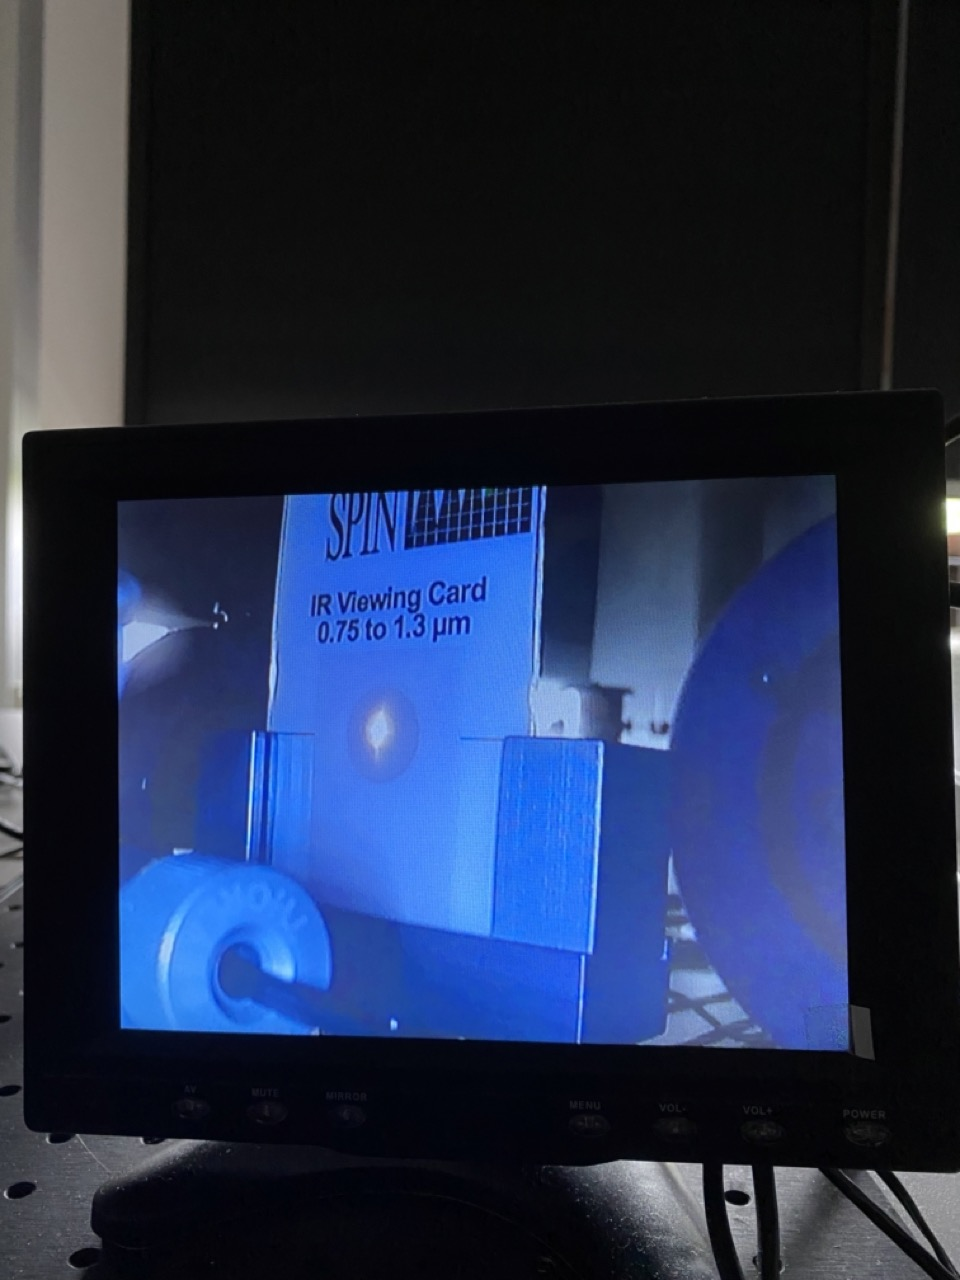
\includegraphics[width=\textwidth]{beam1.jpeg}
        \caption{Diodelaser works as a LED.}
    \end{subfigure}
    \hfill
    \begin{subfigure}[b]{0.45\textwidth}
        \centering
        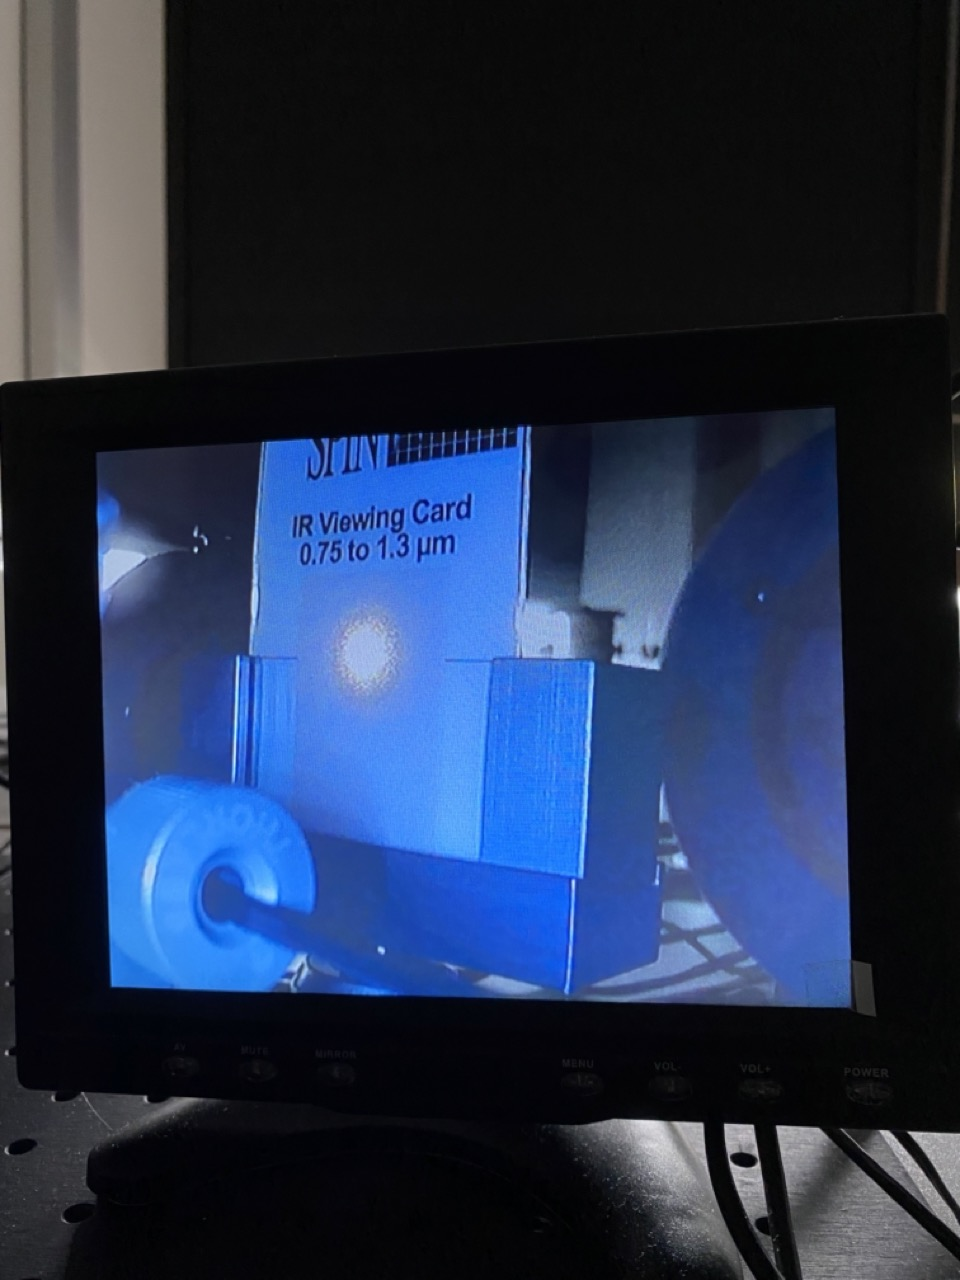
\includegraphics[width=\textwidth]{beam2.jpeg}
        \caption{Diodelaser working as a laser.}
    \end{subfigure}
\end{figure}

\subsection{Rubidium fluorescence}
The fluorescence light of the Rubidium is emitted along the laser beam. This can be observed in the picture
\ref{fig:ffl}. The yellow horizontal line is the light of interest, the lower one is just a reflection
which ocured by the angle 

\begin{figure}
    \centering
    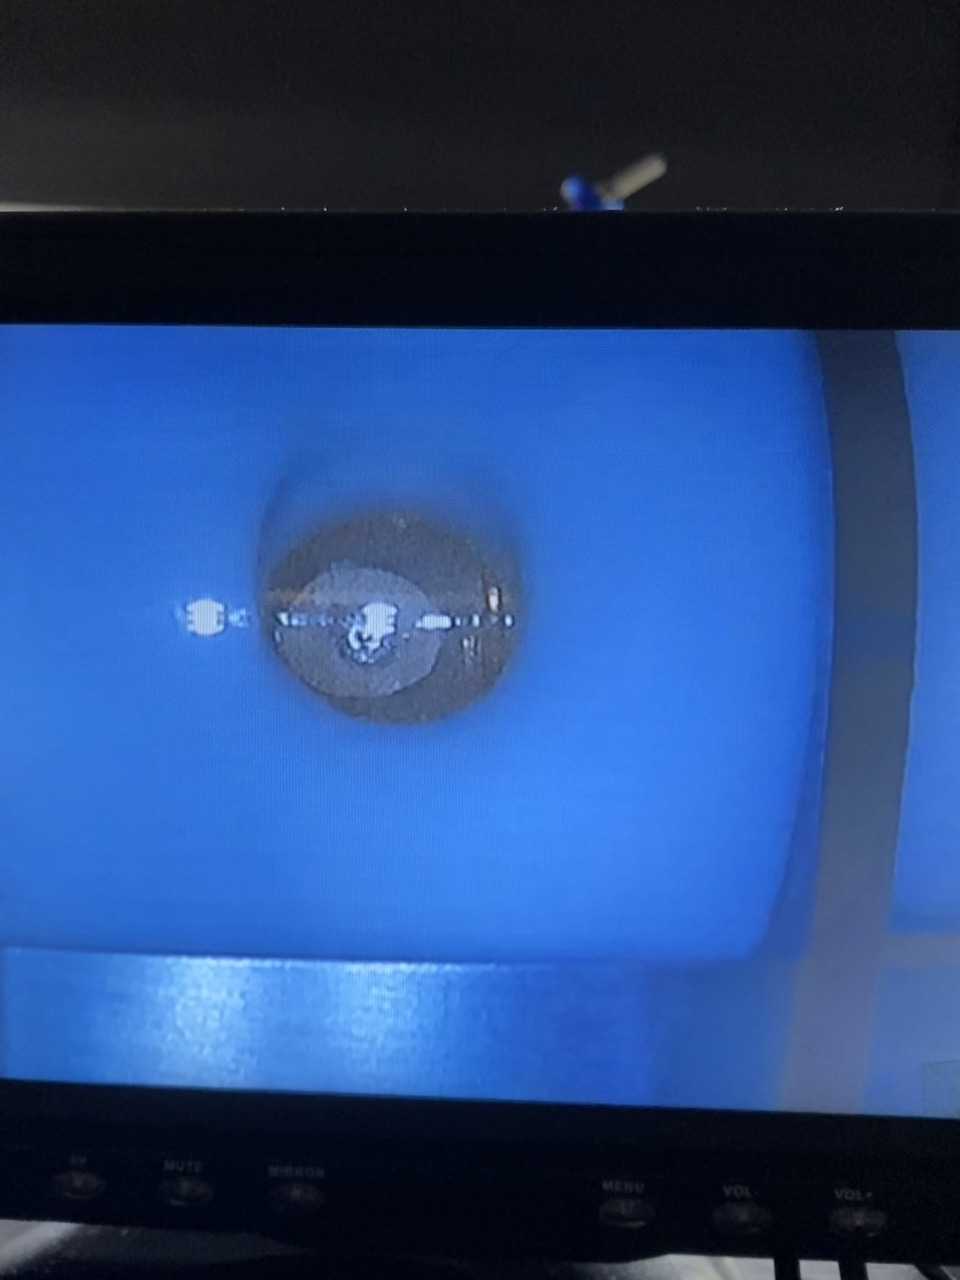
\includegraphics[width=\textwidth]{fl.jpeg}
    \caption{Foto of the rubidium fluorescence.}
\end{figure}

\subsection{Rubidium absorption spectrum}

